%
% fig-torushomologie.tex
%
% (c) 2025 Prof Dr Andreas Müller
%
\begin{figure}
\centering
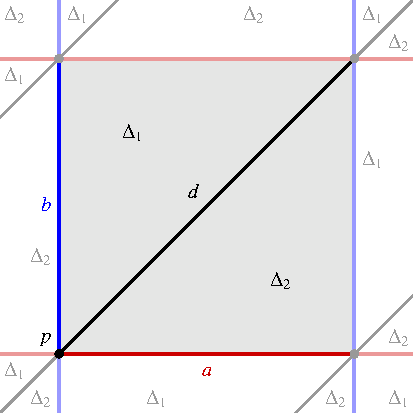
\includegraphics{chapters/120-topologie/images/torushomologie.pdf}
\caption{Triangulation eines Torus mit genau einer Ecke $p$, drei
Kanten $a$, $b$ und $d$ und zwei Dreiecken $\Delta_1$ und $\Delta_2$.
Die Kanten gleicher Farbe sind jeweils miteinander zu identifizieren,
sie entsprechen den Kurven gleicher Farbe in
Abbildung~\ref{buch:topologie:intro:fig:torus}.
\label{buch:topologie:euler:fig:torushomologie}}
\end{figure}
